Physicians use different sources of images in order to make a diagnostic. In the last two decades, many studies have been made in order to automatise the identification and the characterisation of disease by extracting relevant information from those sources of images like the MRI, the Elastography or the Echography, in order to propose help to diagnostic \cite{tartare2014contribution}, \cite{schmitt2011characterization}, \cite{schmitt2013shear}, \cite{ophir1991elastography}.

In \cite{tartare2014contribution}, a new methodology was proposed in order to realise an automatic segmentation of tumour tissues for prostate cancer. Our objective is to generalise and modify the previously proposed method to improve the segmentation of MRI images to diagnose brain pathologies.

Our project focuses on the perfusion MRI by using a spectral clustering algorithm. Physicians use perfusion MRI in order to check the variation of pixel intensity of the MRI image and identify abnormal behaviour. To apply similar methodology, we have to develop a unsupervised classification approach. The main issue is that many classification algorithms like the k-means are not suitable for signal classification. The main purpose of spectral clustering is to firstly estimate the similarity among signals and, build a similarity matrix and work on the eigenvector and eigenvalue of this matrix in order to perform a classification. Spectral clustering algorithms are the most adapted for the data we are dealing with.

This study is the result of a collaboration among four institutes: ENSTA Bretagne, Brest Hospital university Research Center (CHRU), INSERM of Lille and ULCO.

We apply our approach on a perfusion MRI database of twelve patients showing different pathologies in the brain in order to apply our algorithm.Those MRI have been provided by the Brest CHRU. An example of MRI images obtained can be seen in the figure \ref{fig:diffusion}. For each pixel, a variation of the intensity on the different MRI images can be observe.

\begin{figure}
\centering
\begin{subfigure}[t]{0.22\textwidth}
\centering
    \vspace{0.00\textheight}
    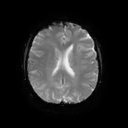
\includegraphics[scale=0.9,angle=0]{Im1.png}
    \caption{MRI without contrast product}
    \label{fig:without} 
\end{subfigure}
\begin{subfigure}[t]{0.22\textwidth}
\centering
    \vspace{0.00\textheight}
    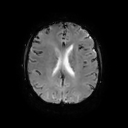
\includegraphics[scale=0.9,angle=0]{Im7.png}
    \caption{beginning of the diffusion}
    \label{fig:First} 
\end{subfigure}
\begin{subfigure}[t]{0.22\textwidth}
\centering
    \vspace{0.00\textheight}
    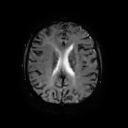
\includegraphics[scale=0.9,angle=0]{Im8.png}
    \caption{Peak of diffusion}
    \label{fig:Second} 
\end{subfigure}
\begin{subfigure}[t]{0.22\textwidth}
\centering
    \vspace{0.00\textheight}
    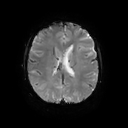
\includegraphics[scale=0.9,angle=0]{Im13.png}
    \caption{end of the diffusion}
    \label{fig:Last} 
\end{subfigure}
    \caption{Diffusion of the contrast product on the MRI.}
    \label{fig:diffusion} 
\end{figure}

%At the beginning, we wanted to apply those results for detection and the characterisation of the thrombus and the deep venous thrombosis. Many options are studied in order to achieve this goal like the use of Elastography and echography \cite{schmitt2011characterization}, \cite{schmitt2013shear}, \cite{ophir1991elastography}.We wanted to apply this methodology which use the MRI images as a new source of information on the clot. Nevertheless, we arrived quickly to those results:
%
%\begin{itemize}
%
%\item The MRI signature of the clot is highly dependent on its age, its composition and surrounding tissues.
%
%\item The position of the clot is not fixed. The clot can be naturally dissolved. 
%
%\item The composition of the clot can be known only through an extraction from the patient, which is not always possible. 
%
%\end{itemize}


